Some words go here

\begin{figure}[htb]
	\centering
	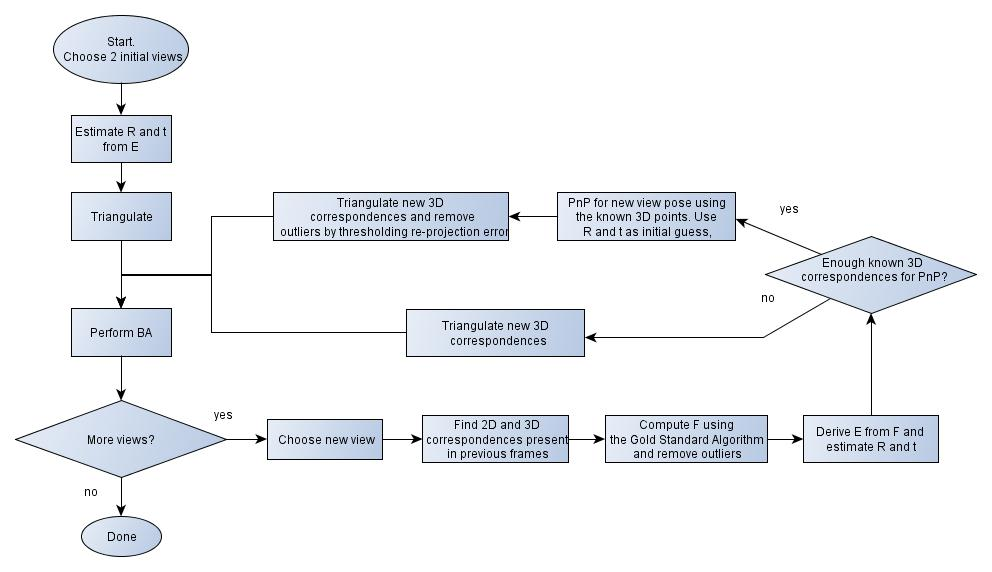
\includegraphics[width=160mm]{images/example1.jpg}
	\caption[This text ends up at the list of figures]{\textit{Data flow between modules.(example image)}}
	\label{fig:block_overview_fig}  %Skapar referens till figuren
\end{figure}


\subsection{Description}
The software part of the system will perform all the image processing and analysis needed to detect usage of a room. In order to make future development of the system easier the software will be written to be as modular as possible. In order to maintain robustness in the system a set of automatic tests will be developed, to prevent regression of the system performance.
 
\subsection{External dependencies}
The software will be written using the OpenCV library to handle the image processing, and where possible interfacing with cameras. Any visualization and debugging tools will be written using the Qt framework.

Cmake will be required to build the source code into an executable.

\subsection{Compatibility}
The software will be possible to compile and run on most major platforms (Windows/OS X). The system will expose and API that allows modules for arbitrary cameras to be written.

The system must be cabable of communicating using a REST API.

\subsection{Limitations}
For integrity reasons no personally identifiable information can be stored or reported by the system.

\subsection{Software Requirements}
\label{sec:software_req}
\reqtable
{	
	\addreq{The system runs on Windows based plattforms}{1}
	\addreq{The system runs on OS x}{1}
	\addreq{The system is modular with respect to the camera manufacturer and/or network API}{1}
	\addreq{The system must not store image data}
}